
\begin{figure}
    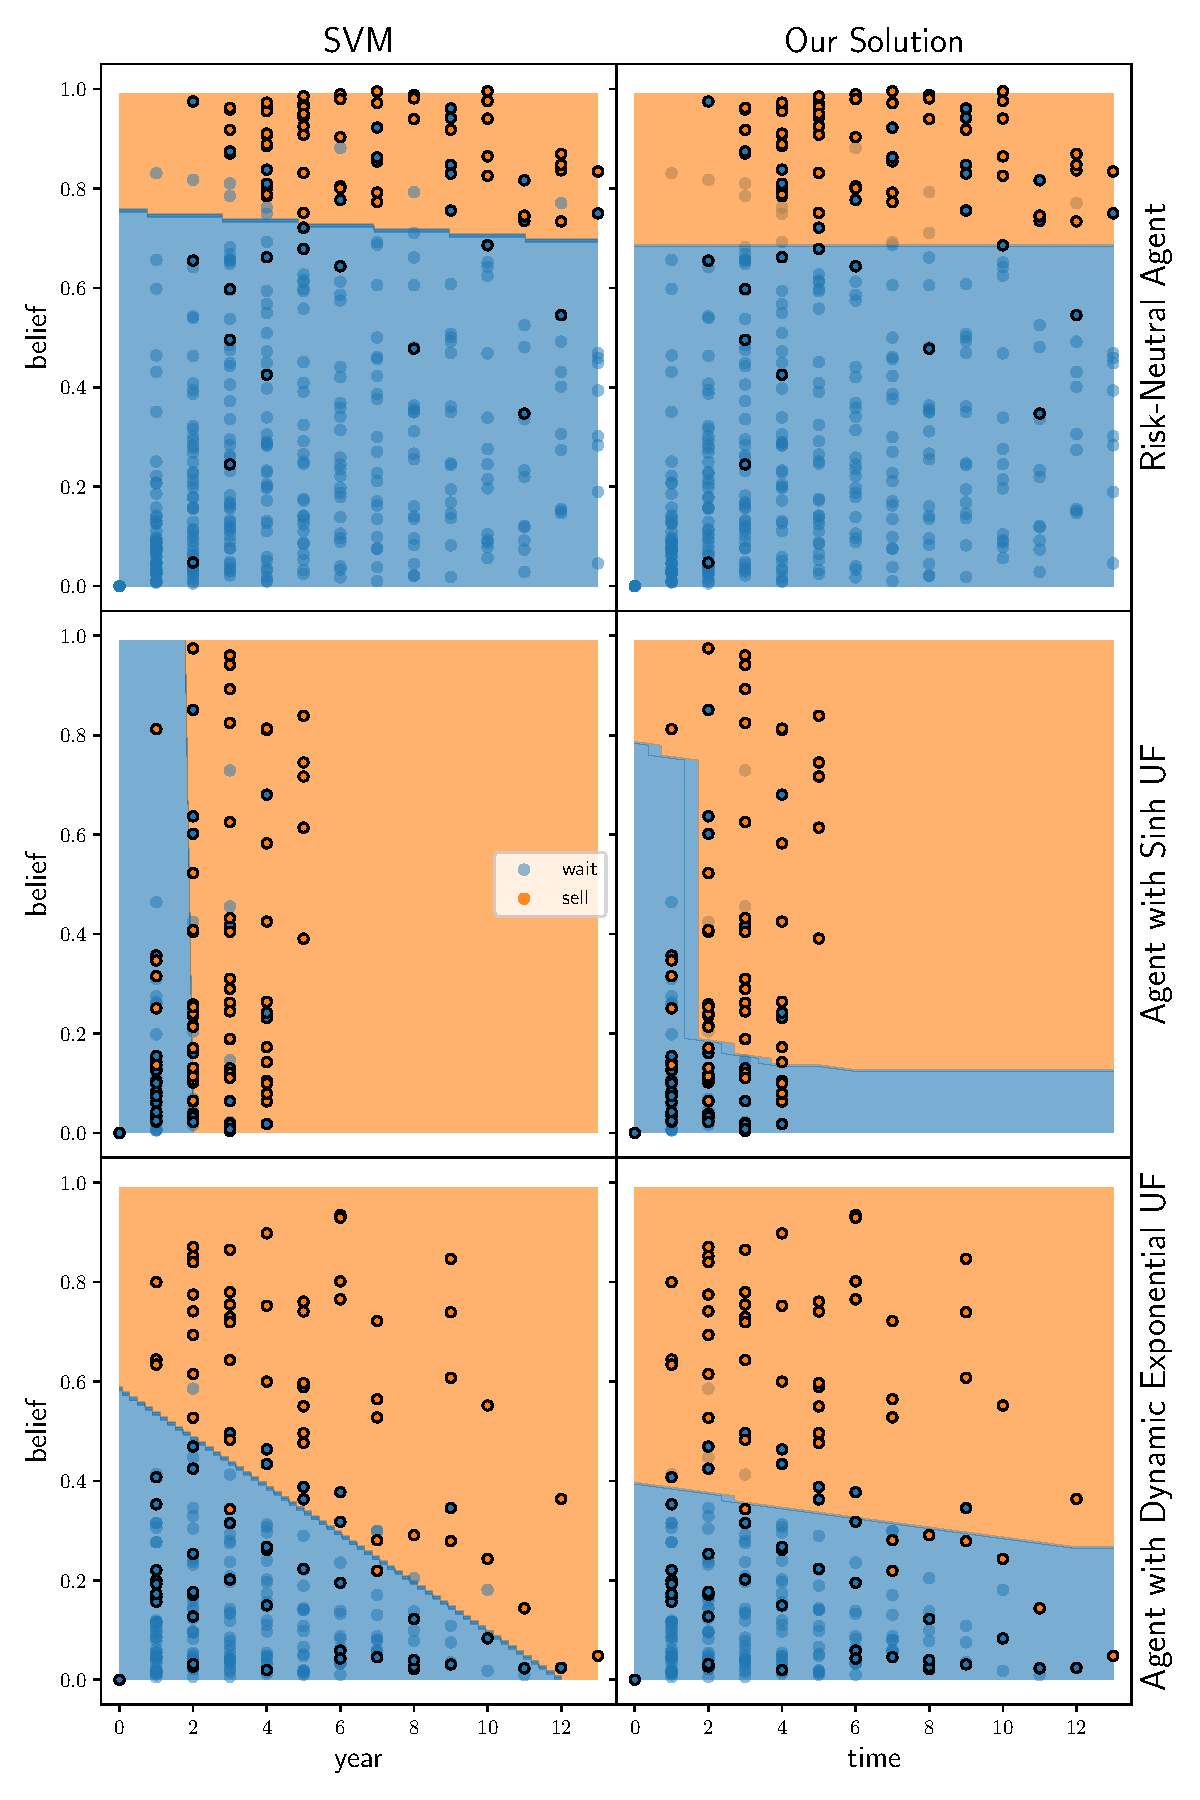
\includegraphics[width=0.8\linewidth]{img/fit}
    \caption{Examples from three human behaviors distinctly observed and replicated with RL agents. Behaviours by row: 1) Constant belief threshold, modelled by exponential utility, 2) Fixed time threshold, modelled by sinh utility, 3) mixed strategy, modelled by dynamic exponential utility. // Left column shows empirical optimal split of data using cross validation and linear kernel support vector machines, right column shows optimal policy found via gridsearch.}
\end{figure}

% TODO 6 boxes with only expensive expert and 3 behavior clusters.

\begin{figure}
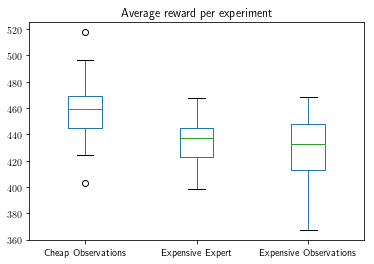
\includegraphics[width=0.4\linewidth]{img/avg_reward.png}
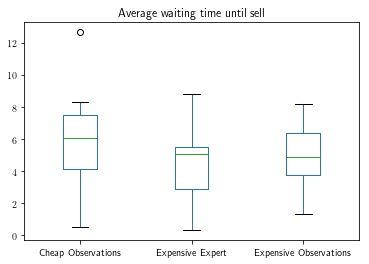
\includegraphics[width=0.4\linewidth]{img/avg_waiting.png}
\caption{Average reward and waiting times in different experiment scenarios.}
\end{figure}
